%---- Sample WMSU BSMATH BEAMER template ------
%---- Begin editing after PREAMBLE END at line 77------
%---- Created by: Christle Jude L. Maquilan - April 2022 --
%---- @jmaq03.jm@gmail.com -----

\documentclass[xcolor=dvipsnames,envcountsect]{beamer}

%------------------------------------------------
%------------------------------------------------
%------------------------------------------------
%------------------------------------------------
%------------------------------------------------
%----------▼▼▼▼▼ START PREAMBLE ▼▼▼▼▼----------

%-------- theme --------
\usetheme{Madrid}

%-------- color --------
\definecolor{crimsonred}{RGB}{153,0,0} % Official RGB code for Crimson Red
\definecolor{crimsonred2}{RGB}{120,10,10}
\usecolortheme[named=crimsonred]{structure}
%-------- set color of 'example block' to crimson theme --------
\setbeamercolor{block body example}{bg=white}
\setbeamercolor{block title example}{fg=white, bg=red!50!black}
\setbeamercolor{section in head/foot}{bg=crimsonred2,fg=white}

%-------- font --------
\setbeamerfont{structure}{family=\rmfamily,series=\bfseries}
\usefonttheme[stillsansseriftext]{structurebold}
\setbeamerfont{section in head/foot}{size=\tiny}

%-------- misc structure --------
\useoutertheme[footline=authortitle,subsection=false]{miniframes}
\setbeamerfont{footline}{size=\fontsize{8}{11}\selectfont}
\useinnertheme{rounded}
\addtobeamertemplate{block begin}{}{\justifying}
\newtheorem{remark}[theorem]{Remark}
\renewcommand{\indent}{\hspace*{2em}}
\setbeamertemplate{theorems}[numbered]
\setbeamertemplate{caption}[numbered]
\usepackage[justification=centering]{caption}
\renewcommand{\qedsymbol}{$\blacksquare$}

\beamertemplatenavigationsymbolsempty

%-------- packages to be used -------
\usepackage{amsmath,amsfonts,amssymb,amscd,amsthm}
\usepackage{graphicx,xcolor,comment}
\usepackage{mathrsfs} 
\usepackage{multirow}
\usepackage{array}
\usepackage{hyperref}
\usepackage{multicol}
\usepackage{ragged2e}
\usepackage{caption}
\usepackage[french]{babel}
\usepackage{rotating}
\usepackage{enumerate}
\usepackage{tikz}
\usepackage{bm}
\usepackage{csquotes}
\usepackage{wrapfig}
\usepackage{listings}

\usepackage{appendixnumberbeamer}

%-------- for bibliography -----------------
\usepackage{biblatex}
\setbeamertemplate{bibliography item}{\insertbiblabel}
\addbibresource{References.bib}
\setbeamertemplate{frametitle continuation}{\frametitle{\color{white}Bibliographie}}

\makeatletter
\let\beamer@writeslidentry@miniframeson=\beamer@writeslidentry
\def\beamer@writeslidentry@miniframesoff{%
  \expandafter\beamer@ifempty\expandafter{\beamer@framestartpage}{}% does not happen normally
  {%else
    % removed \addtocontents commands
    \clearpage\beamer@notesactions%
  }
}
\newcommand*{\miniframeson}{\let\beamer@writeslidentry=\beamer@writeslidentry@miniframeson}
\newcommand*{\miniframesoff}{\let\beamer@writeslidentry=\beamer@writeslidentry@miniframesoff}
\makeatother


%-------- WMSU Backgound -------------------
%\usebackgroundtemplate{%
%	\tikz[overlay,remember picture] \node[opacity=0.02, at=(current page.center)] {
%		
\includegraphics[height=4.5in,width=4.5in]{./Figures/WMSU LOGO.png}};
%}

%----------▲▲▲▲▲ PREAMBLE END ▲▲▲▲▲----------
%------------------------------------------------
%------------------------------------------------
%------------------------------------------------
%------------------------------------------------
%------------------------------------------------

%---------START EDITING HERE---------------------
\title[Études des systèmes GNSS des smartphones]{Études des systèmes GNSS des smartphones}

\author [Noë Charlier - n°52340]{\textbf{Noë Charlier}}

\institute[Lycée Paul Constans] {\emph{Professeurs: }\textbf{C. Delacour, M. Petitcuenot}\\[1em]
	Classe préparatoire aux grandes écoles\\PT\\Lycée Paul Constans\\[1em]

\includegraphics[scale=0.4]{./Figures/logo Paul Constans.jpg}}

\date[2022 - 2023]{\footnotesize TIPE - \textbf{2022, 2023} - N°\textbf{52340}}
%--------- START DOCUMENT ------------------
\begin{document}
	
\begin{frame}{\titlepage}\end{frame}
%--------- Sujet et Domaine ----------------------
\section{Introduction}
\begin{frame}
	\frametitle{Introduction}
		\justifying
		\textit{Besoin grandissant de solution GNSS:}
		\begin{figure}
			\centering
			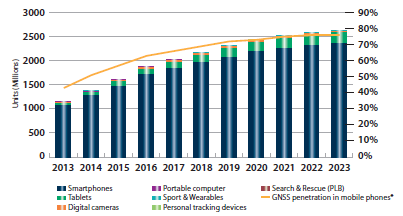
\includegraphics[scale=0.8]{./Figures/stats.png} \\
			\caption {Appareils GNSS par plate-forme. \cite{marketreport}}
		\end{figure}
\end{frame}
\begin{frame}
	\frametitle{Définition GNSS}
		\justifying
		\textbf{GNSS:} \textit{Global Navigation Satellite System} (Système de navigation par satellite global)\\
		%Constellation de satellites permettant de localiser un point sur la Terre.
		\begin{figure}
			\centering
			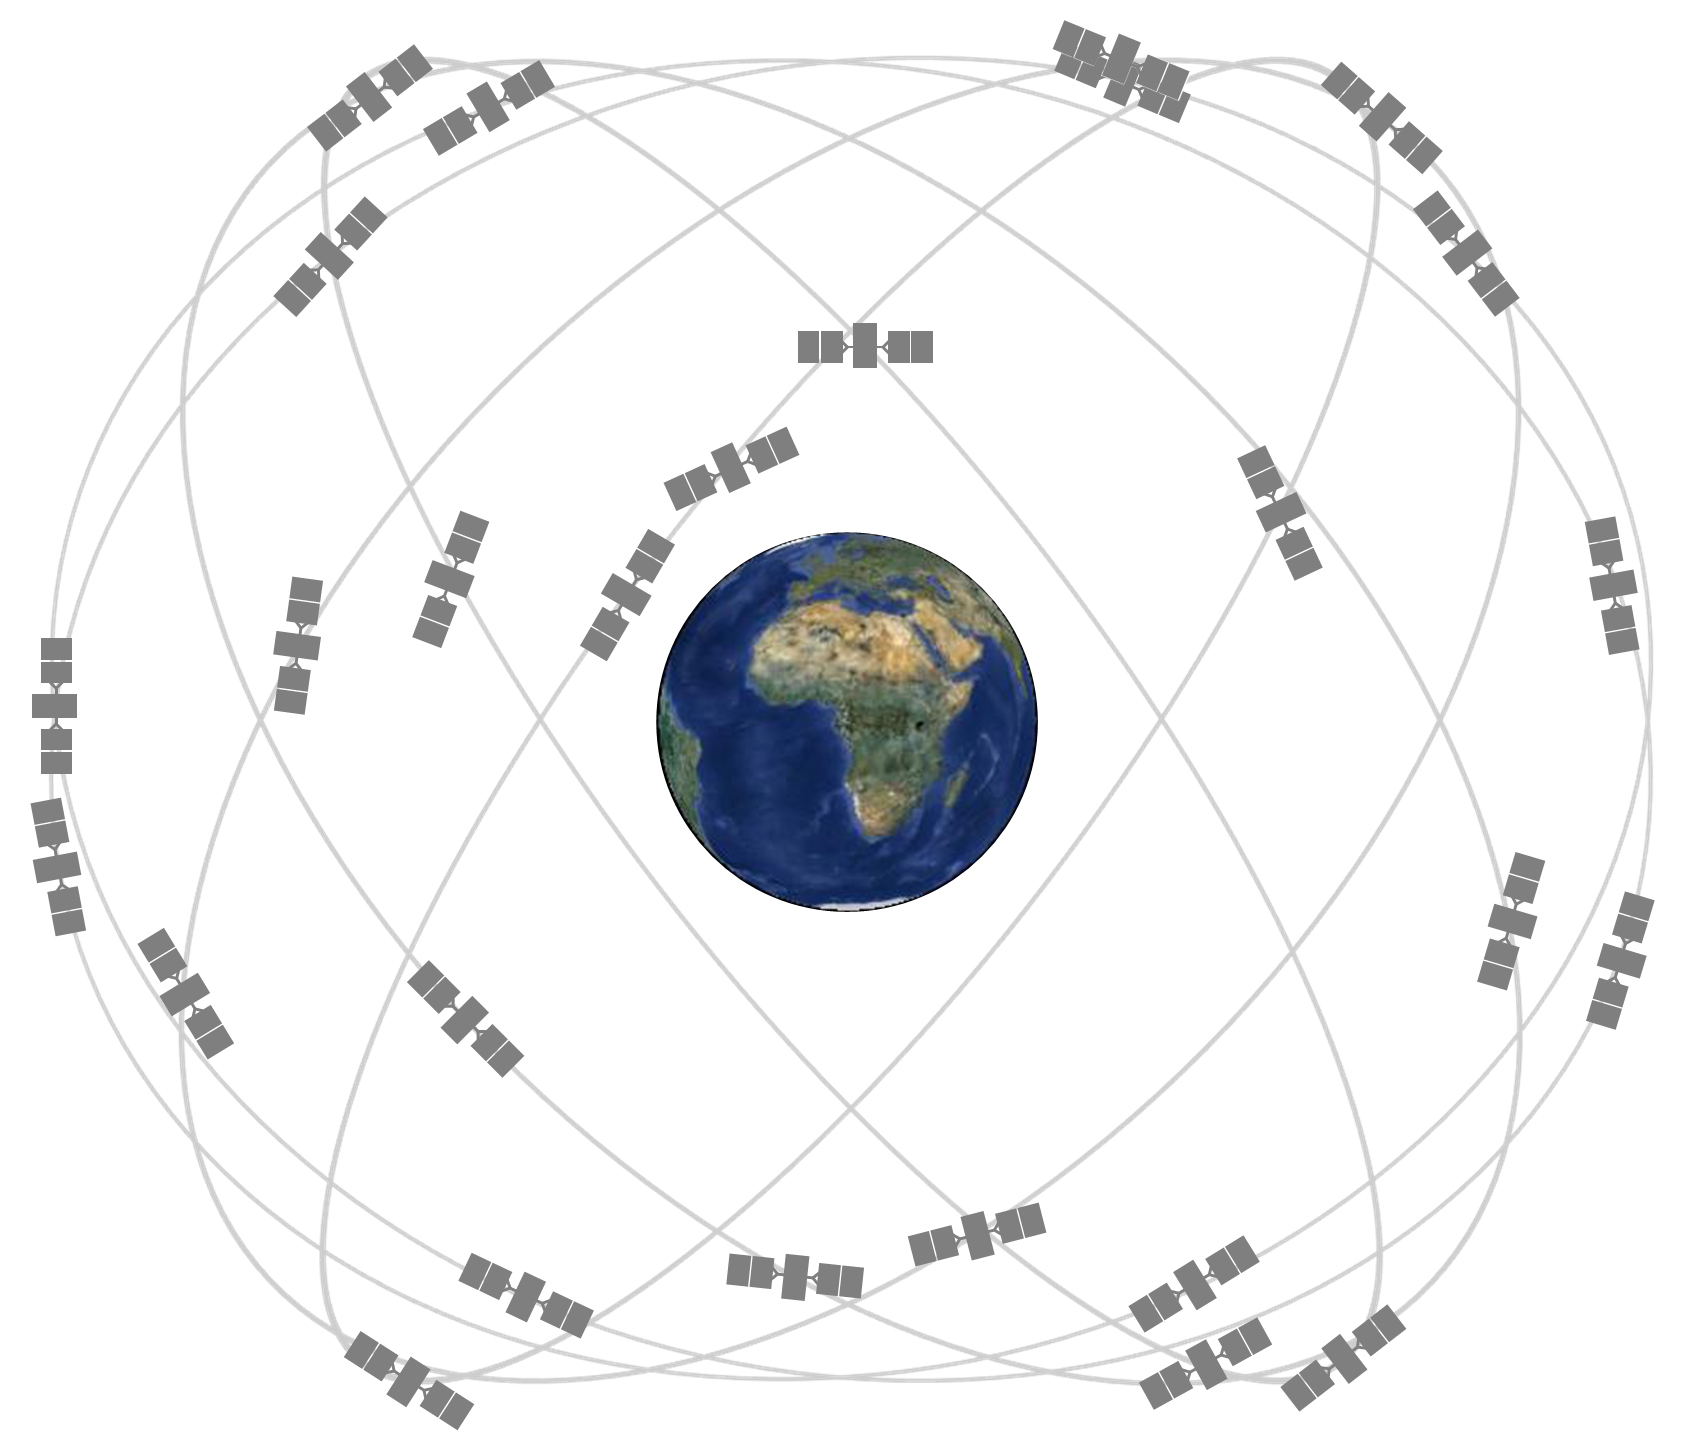
\includegraphics[width=0.3\textwidth]{./Figures/constellation.jpg} \\
			\caption {Système de navigation par satellite global. \cite{cons}}
		\end{figure}
\end{frame}

\begin{frame}
	\frametitle{Fonctionnement du GPS}
	\justifying
	\begin{columns}

		\begin{column}{0.5\textwidth}
			\begin{figure}
				\centering
				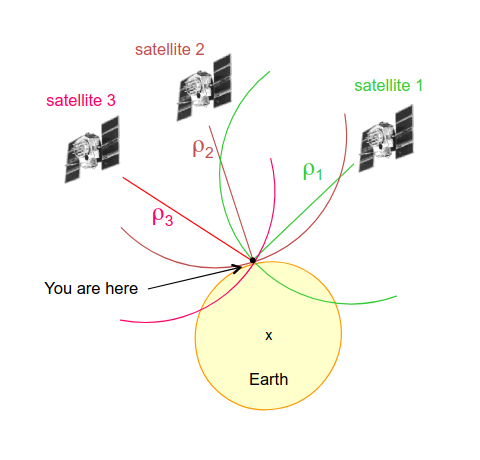
\includegraphics[width=0.9\textwidth]{./Figures/ENS_gnss.png} \\
				\caption {Fonctionnement du GPS. \cite{ens}}
			\end{figure}
		\end{column}

		\begin{column}{0.5\textwidth}
			Une sphère de rayon $\rho_1 = (\Delta t_1 \cdot c) $ \\
			3 satellites, intersection des 3 sphères.
			\newline
			Et donc {\footnotesize$\rho_s^s = \sqrt{(X^s-X_r)^2 + (Y^s-Y_r)^2 + (Z^s-Z_r)^2}$} \\
			Avec:
			\begin{itemize}
				\item $X^s, Y^s, Z^s$ : coordonnées du satellite $s$ ;
				\item $X_r, Y_r, Z_r$ : coordonnées du récepteur.
			\end{itemize}
		\end{column}

	\end{columns}

\end{frame}

\begin{frame}
	\frametitle{Sources d'incertitude}
	\justifying
	\begin{itemize}
		\item Les horloges des satellites et des récepteurs ne sont pas synchronisés. ($\delta t$) {\tiny (Exemple Annexe 6)}
		\item Réfraction lors de la propagation dans l’atmosphère :
		\item \begin{enumerate}
			\item Troposphérique %(dépend de la température et de la pression atmosphérique)
			 ($T_r^s$)
			\item Ionosphérique (dépend de la densité ionique)
			 ($I_r^s$)
		\end{enumerate}
	\end{itemize}
	Modèle plus complet :
	\begin{equation}
		\boxed{R_r^s = \rho_r^s + c\delta t + T_r^s + I_r^s + ...}
	\end{equation}
\end{frame}
\begin{frame}
	\frametitle{Précision des orbites}
	\justifying
	Les systèmes GNSS sont basés sur des orbites prédites émises par les satellites. \\
	Ces \textbf{éphémérides} doivent donc être très précises. 
	%{\small(Perturbation gravitationnelle (cf. Annexe 1))} \\
	\begin{figure}
		\centering
		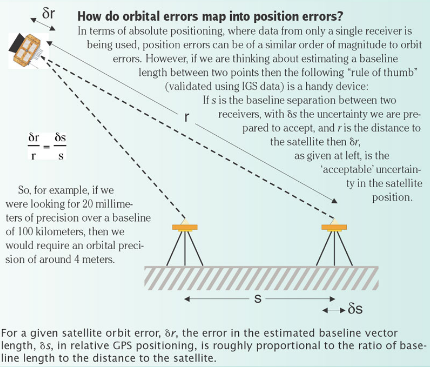
\includegraphics[width=0.35\textwidth]{./Figures/ENS_gnss2.png} \\
		\caption {Précision des orbites. \cite{ens}}
	\end{figure}
	{\small	\textit{Il existe aussi des services qui recalculent les éphémérides apostériori. (eg. IGN)}}
\end{frame}
\begin{frame}
	\frametitle{Multipath et dilution}
	\justifying
	\begin{columns}
		\begin{column}{0.5\textwidth}
			Le \textbf{multipath} (multi-trajet): le signal émis par le satellite est réfléchi 
			%par un objet 
			avant d'atteindre le récepteur. (cf. Figure \ref{fig:multipath})
			\begin{figure}
				\centering
				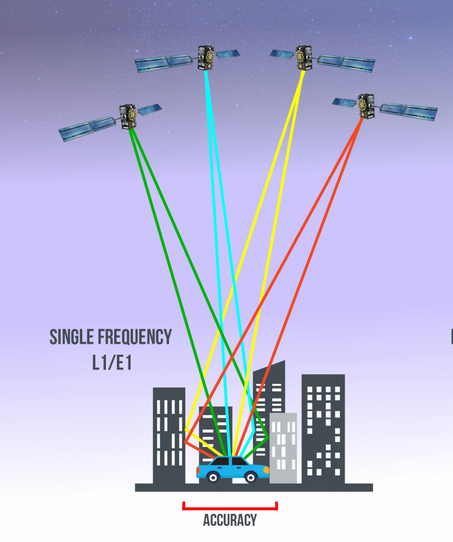
\includegraphics[width=0.5\textwidth]{./Figures/multipath.png} \\
				\caption {Multipath \cite{esa}}
				\label{fig:multipath}
			\end{figure}
		\end{column}
		\begin{column}{0.5\textwidth}
			La \textbf{dilution} (GDOP): la géométrie des satellites influe sur la précision. (cf. Figure \ref{fig:dilution})
			% par rapport au récepteur influe sur la précision de la mesure. (cf. Figure \ref{fig:dilution})
			\begin{figure}
				\centering
				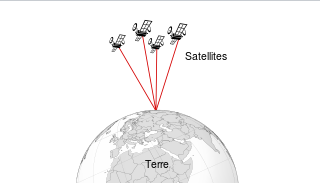
\includegraphics[width=0.8\textwidth]{./Figures/dilution.png} \\
				\caption {Coef. de dilution élevée \cite{esa}}
				\label{fig:dilution}
			\end{figure}
			
		\end{column}
	\end{columns}
\end{frame}

\begin{frame}{\frametitle{Sommaire}\tableofcontents}\end{frame}

\begin{frame}
	\frametitle{Problématique}
	\centering
	\begin{block}
		\scshape
			\begin{center}
				\Huge\emph{Comment peut-on réduire l'impact de l'urbanisation sur les systèmes GNSS pour améliorer la
				précision de la géolocalisation par satellite ?}
			\end{center}
	\end{block}
\end{frame}

\begin{frame}
	\frametitle{Objectifs}
	\justifying
	\begin{enumerate}
		\item Impact de l'ionosphère et des corrections possibles. \\
		\item Étude du multipath, dilution géométrique, GPS à doubles fréquences. \\
		\item Comparaison Ville / campagne de la précision.	
	\end{enumerate}
\end{frame}
%---------- DEFINITION/PRELIMINARY ---------------------
\section{L'ionosphère}
\begin{frame}
	\frametitle{Définition}
	\begin{columns}
	    \justifying
		\begin{column}{0.5\textwidth}
	    	\textbf{L'ionosphère :} 
			%L'ionosphère est la couche de l'atmosphère 
			Située entre \textbf{60 et 1000 km} d'altitude. \\
			Constituée de particules chargées électriquement, les ions, en mouvement.
		\end{column}
		\begin{column}{0.5\textwidth}
			\begin{figure}
				\centering
				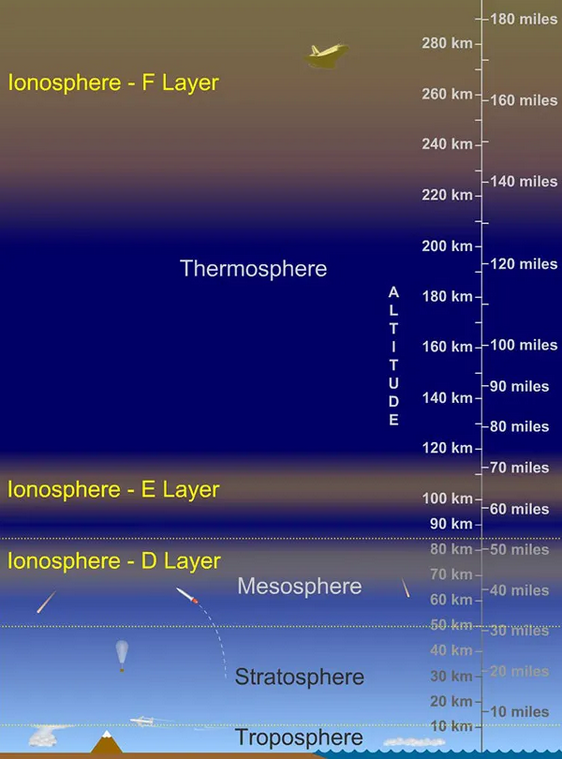
\includegraphics[width=0.7\textwidth]{./Figures/iono_ucar.png}
				\caption {Régions de l'ionosphère \cite{ucar}}	
			\end{figure}
		\end{column}	
	\end{columns}
\end{frame}
\begin{frame}
	\frametitle{Impact sur la propagation}
		\justifying
		\begin{columns}
			\begin{column}{0.5\textwidth}
				\textbf{Impact sur la propagation :} \newline
				\begin{itemize}
					\item \textbf{Propagation directe} - \textbf{Sans} interaction avec l'ionosphère. \newline
					\item \textbf{Propagation réfractée} - \textbf{Avec} interaction avec l'ionosphère.
				\end{itemize}
				\begin{center}
					{\small Indice : \\ $n=1- \frac{f_p^2}{2f^2} < 1$}
				\end{center}
				\begin{flushright}
					{\tiny (Voir annexe 2)}
				\end{flushright}
			\end{column}
			\begin{column}{0.5\textwidth}
				\begin{figure}
					\centering
					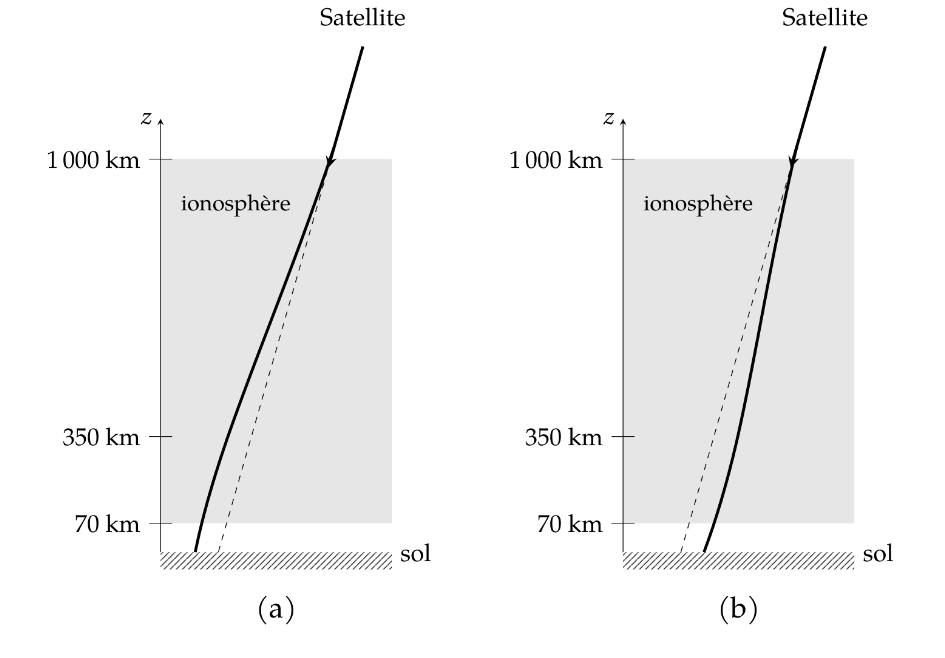
\includegraphics[width=0.6\textwidth]{./Figures/iono_e3a.png}
					\caption {Propagation directe et réfractée \cite{e3a}}
				\end{figure}
			\end{column}
	\end{columns}
\end{frame}
\begin{frame}
	\frametitle{Quelle erreur ?}
	\justifying
		\begin{columns}
			\begin{column}{0.5\textwidth}
				\begin{figure}
					\centering
					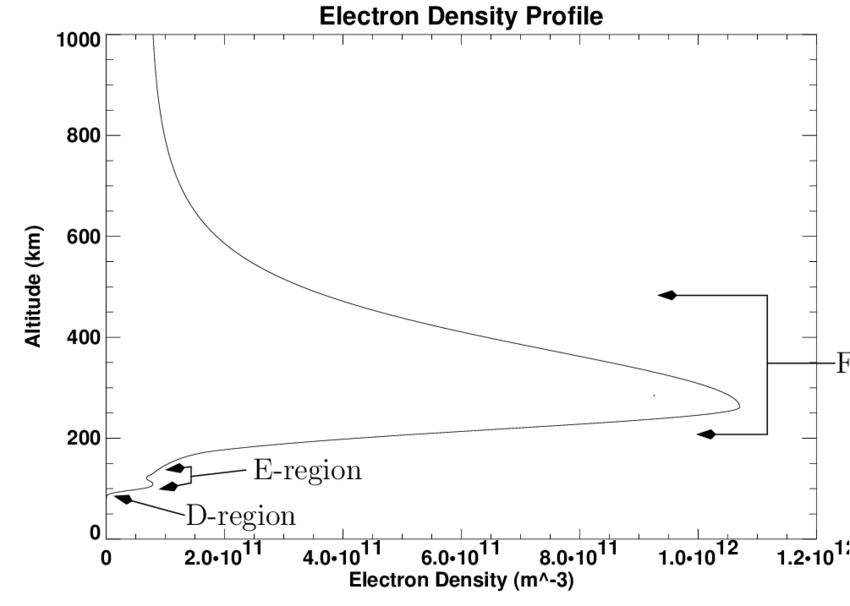
\includegraphics[width=1\textwidth]{./Figures/iono_profil.png}
					\caption {Profil Ionosphérique \cite{ionoprofil}}
				\end{figure}
			\end{column}
			\begin{column}{0.5\textwidth}
				{\tiny \textit{Milieu Linéaire, Isotrope, transparent, inhomogène}}\\
				Retard Ionosphérique : \\
				$\tau = \frac{1}{c} \int_{0}^{H_0} (\frac{c}{v_g}-1)$ \newline

				Erreur de distance : \\
				$L = \frac{a}{f_1^1} C_{ET}$ avec $C_{ET} = \int_{0}^{H_0} n_e dz$ (Contenu Électronique Total)
				\newline

				\begin{center}
					\textbf{A un TEC de }$1.5\cdot 10^{17} m^{-2}$, \boxed{$L = 220m$}
				\end{center}

				On a besoin de la \textbf{phase} et de la \textbf{pseudorange} sur deux fréquences.
				\begin{flushright}
					\tiny{(Voir Annexe 2)}
				\end{flushright}
			\end{column}
		\end{columns}
\end{frame}

\begin{frame}{GPS à doubles fréquences}
	\justifying
	\textbf{Afin de calculer le TEC, un récepteur Dual-Band (L1, L5) est nécessaire :}
	\newline
	\begin{columns}
		\begin{column}{0.5\textwidth}
			\begin{figure}
				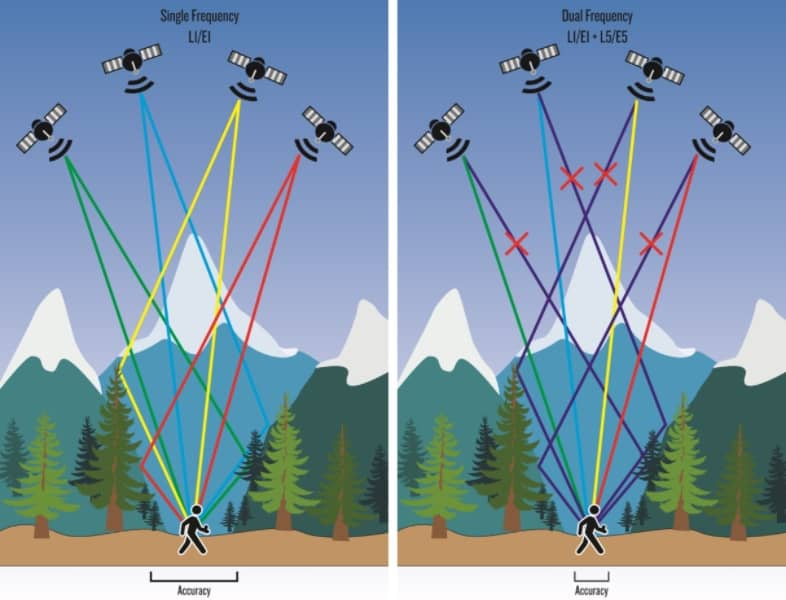
\includegraphics[width=0.9\textwidth]{./Figures/dual_band.jpg}
				\caption{\textit{Image: Garmin}}
			\end{figure}
		\end{column}
		\begin{column}{0.5\textwidth}
			Désormais disponible dans les smartphones(depuis 2018):
			\begin{figure}
				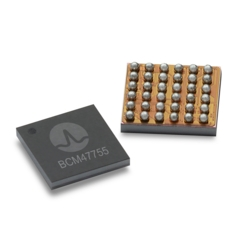
\includegraphics[width=0.7\textwidth]{./Figures/BCM47755.jpg}
				\caption{Broadcom BCM47755, \textit{Broadcom Inc.}}
			\end{figure}
		\end{column}
	\end{columns}
\end{frame}


%----------- MAIN RESULTS ------------------------------
\section{Exp. Ionosphérique}
\begin{frame}
	\centering
	\begin{block}
		\scshape
		\begin{center}
			\Huge Expérimentations Ionosphérique
		\end{center}
	\end{block}
\end{frame}
\begin{frame}{Préambule}
        \textbf{Méthode d'évaluation:} 
		Le retard s'évalue grâce à un même signal sur deux fréquences.

        \textbf{Le signal GPS:} 
	    \begin{itemize}
            \item \textbf{Pseudorange} - La pseudorange (distance) s'évalue à l'aide d'une fonction de corrélation.
            \item \textbf{Phase} - La phase s'évalue sur le nombre de phases depuis le début d'acquisition.
        \end{itemize}
		\begin{flushright}
			\tiny{(Voir Annexe 3)}
		\end{flushright}
		Il est possible de connaître l'état de l'ionosphère (indice Kp).
\end{frame}

\begin{frame}{Protocole expérimental}
	 \begin{columns}
		\begin{column}{0.3\textwidth}
			\begin{figure}
				\centering
				
\includegraphics[width=0.7\textwidth]{./Figures/gnss_logger.jpg}
				\caption {GNSS Logger de \textit{Google}}	
			\end{figure}
		\end{column}
		\begin{column}{0.7\textwidth}
			\begin{itemize}
				\item Récupération des données brute sur Xiaomi Mi 8 avec \textit{GNSS Logger} de \textit{Google}.
				\item Calcul du délai ionosphérique avec \textit{Python} {\tiny (Voir Annexe 7)}.
			\end{itemize}
			\begin{figure}
				\centering
				\includegraphics[width=0.5\textwidth,angle=-90,origin=c]{./Figures/protoc.jpg}
				\caption {Protocole expérimental}
			\end{figure}
		\end{column}
	 \end{columns}
\end{frame}

\begin{frame}{Contexte}
	\begin{columns}
		\begin{column}{0.5\textwidth}
			\begin{figure}
				\centering
				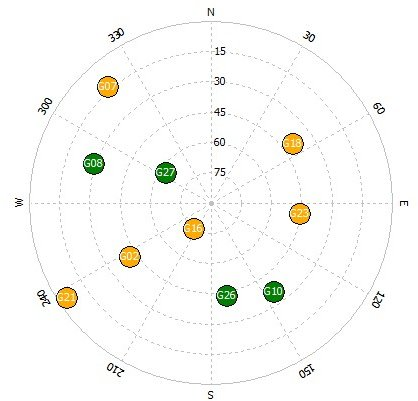
\includegraphics[width=0.9\textwidth]{./Figures/skyplot.jpg}
				\caption {Carte du ciel}
			\end{figure}
		\end{column}
		\begin{column}{0.5\textwidth}
			\begin{figure}
				\centering
				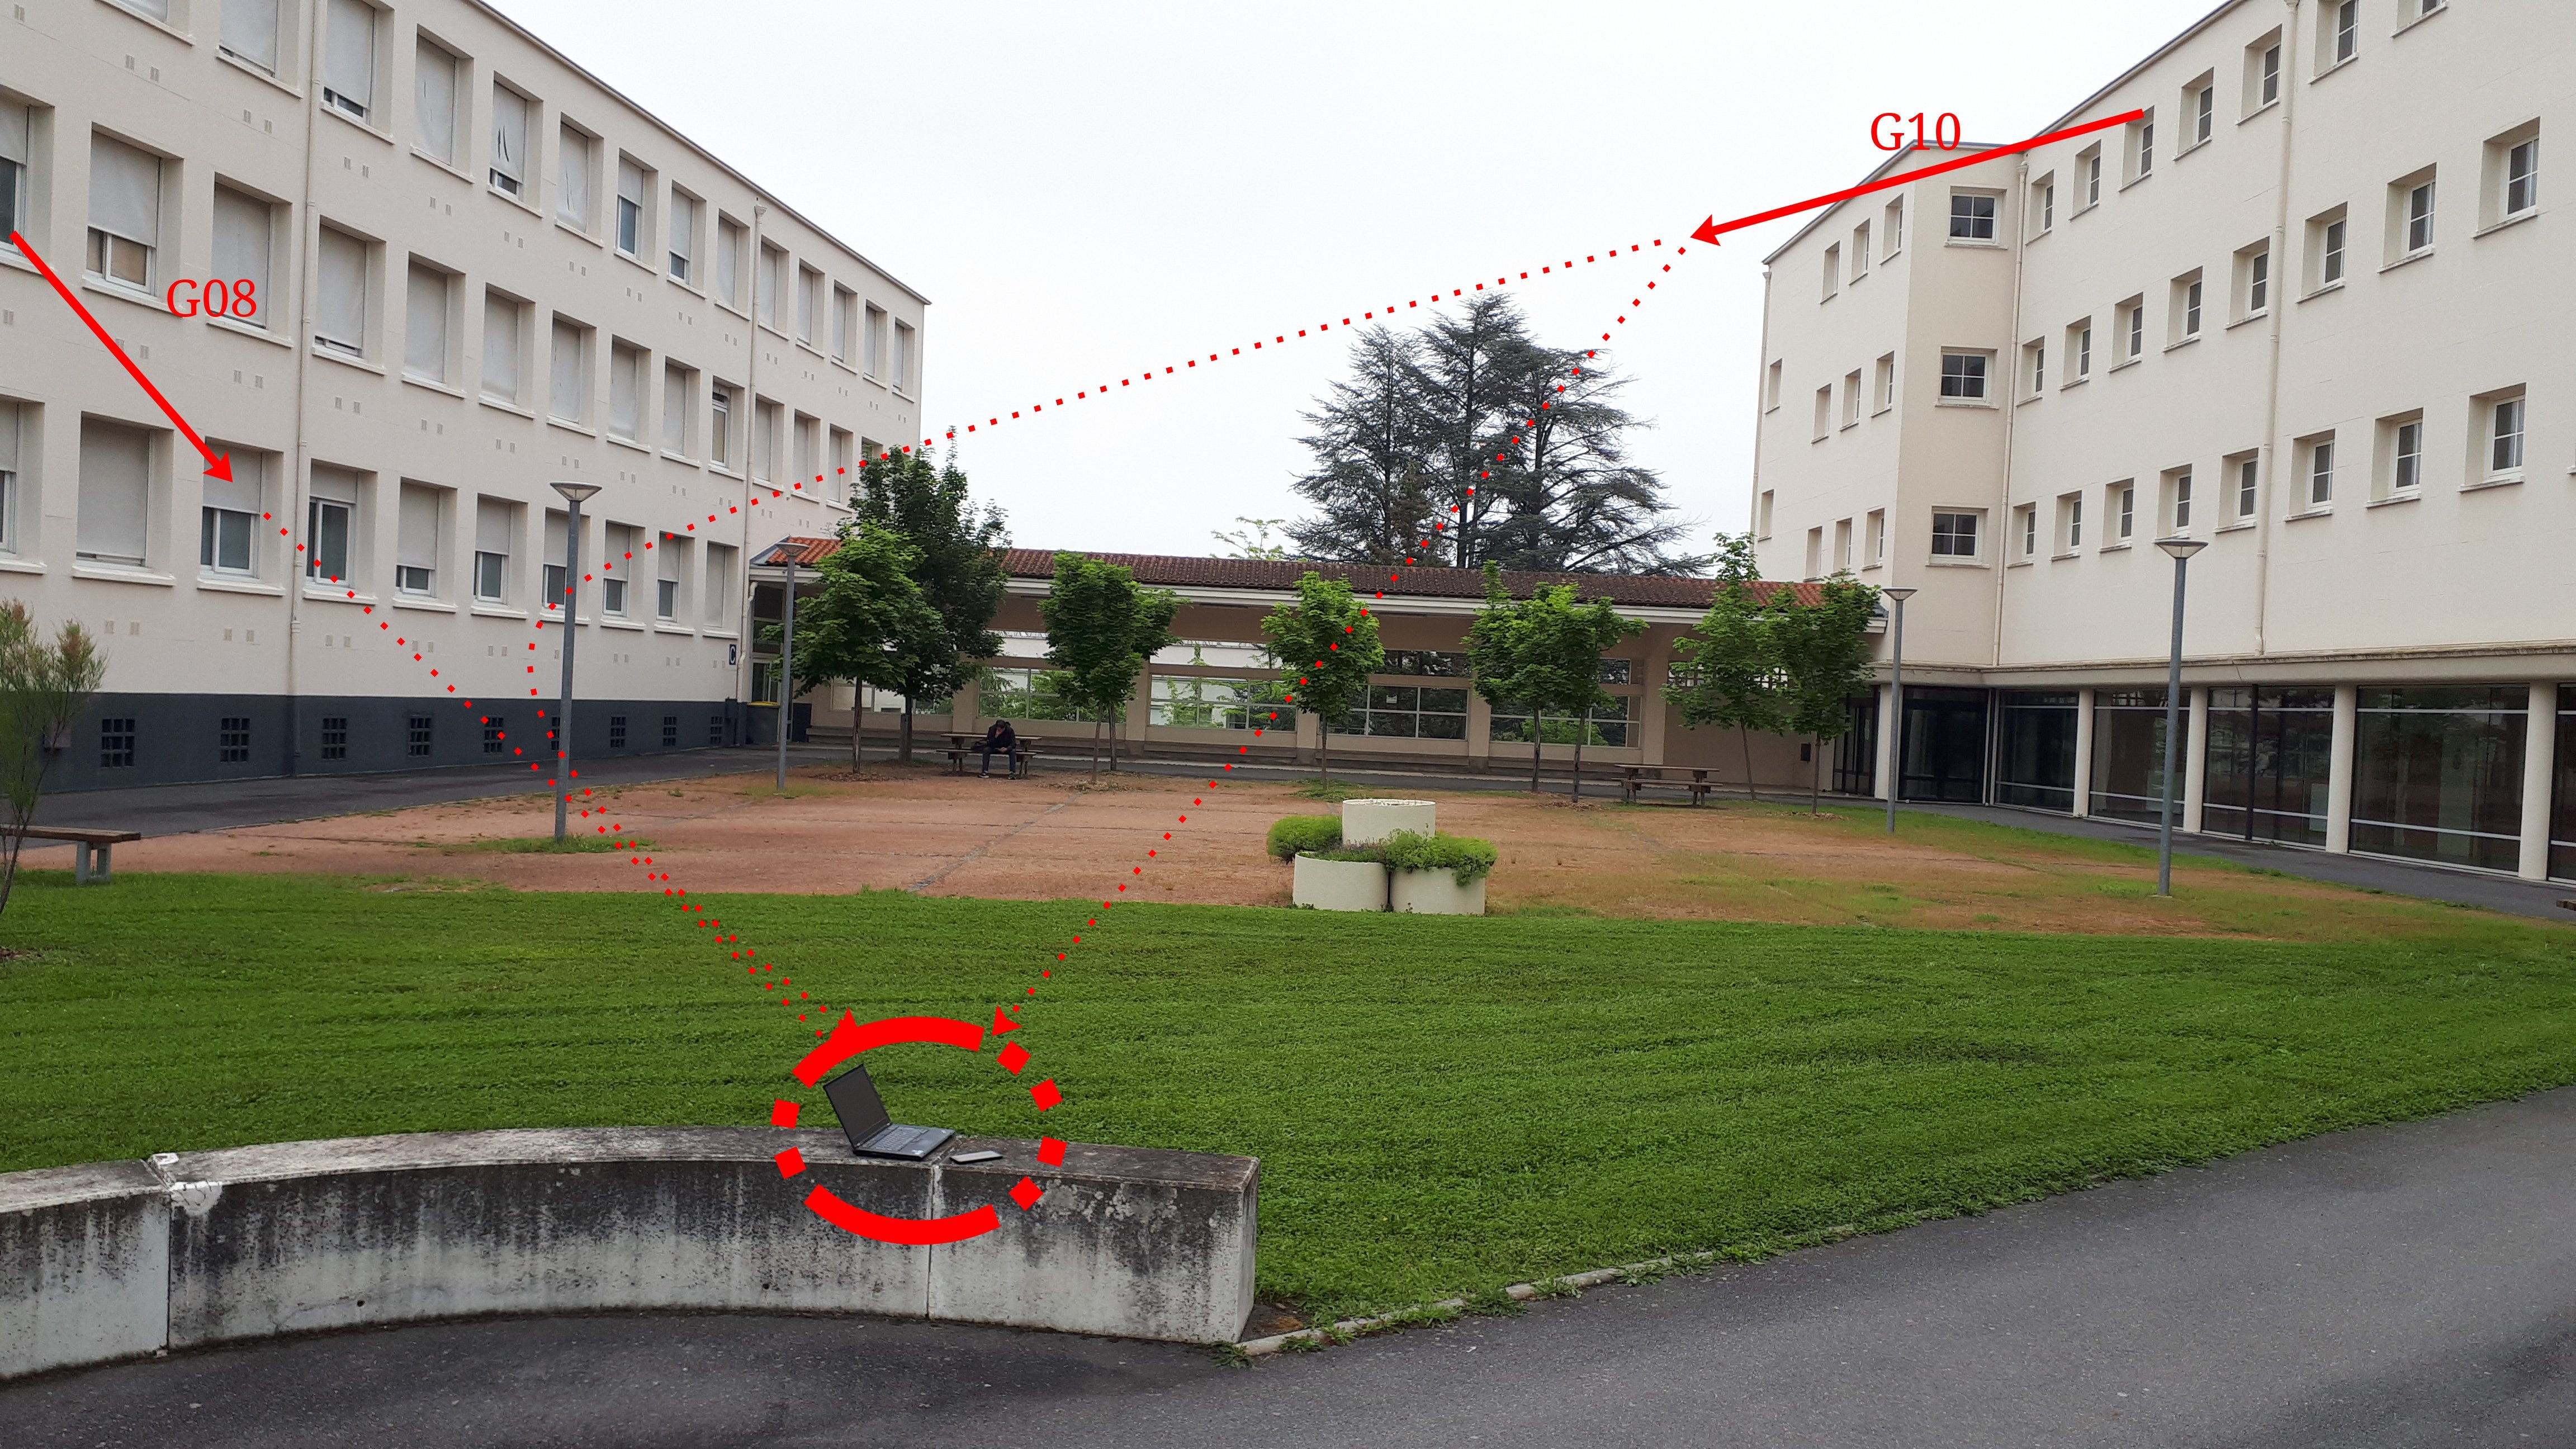
\includegraphics[width=1\textwidth]{./Figures/spot1.jpg}
				\caption {Image de la session 1, Nord sur la gauche}
			\end{figure}
		\end{column}

	\end{columns}
\end{frame}

\begin{frame}{Contexte - Signal sur bruit}
	\begin{columns}
		\begin{column}{0.5\textwidth}
			\textbf{Signal sur bruit :} 
			\begin{itemize}
				\item Rapport entre la puissance du signal et la puissance du bruit.
				\item $SNR = 10 \cdot log_{10}(\frac{P_{signal}}{P_{bruit}})$
			\end{itemize}
			\begin{figure}
				\centering
				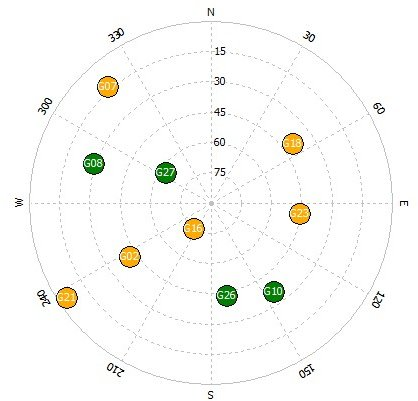
\includegraphics[width=0.6\textwidth]{./Figures/skyplot.jpg}
				\caption {Skyplot}
			\end{figure}
		\end{column}
		\begin{column}{0.5\textwidth}
			% \begin{figure}
			% 	\centering
			% 	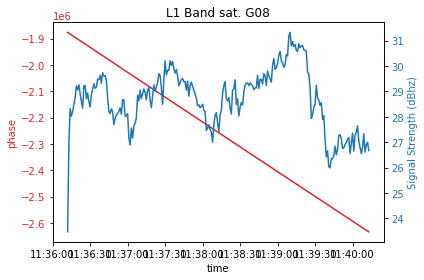
\includegraphics[width=0.6\textwidth]{./Figures/G08_L1.png}
			% 	\caption {Signal sur bruit G08}
			% \end{figure}
			\begin{figure}
				%\centering
				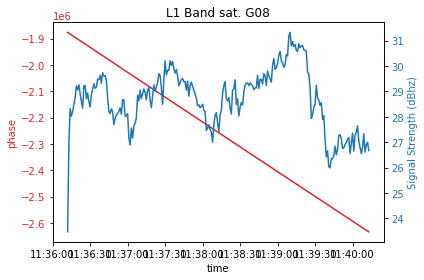
\includegraphics[width=0.8\textwidth]{./Figures/G08_L1.png}
				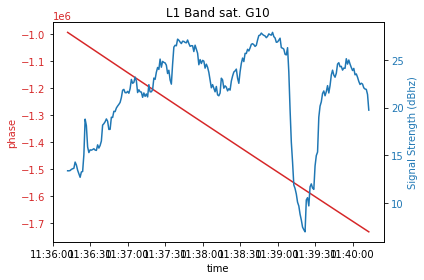
\includegraphics[width=0.8\textwidth]{./Figures/G10_L1.png}
				%\caption {Signal sur bruit G10}
				\caption {SNR, G08 et G10}
			\end{figure}
		\end{column}
	\end{columns}
\end{frame}

\begin{frame}{Résultats}
	L'estimation du délai n'est possible que sur de courte session due aux \textit{duty cycle} {\tiny (Voir Annexe 3)}
	\begin{columns}
	\begin{column}{0.5\textwidth}
		\begin{figure}
			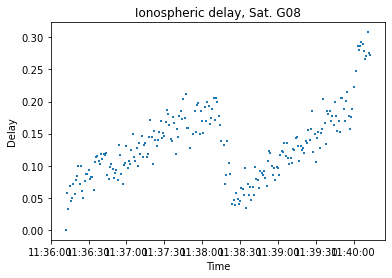
\includegraphics[width=0.9\textwidth]{./Figures/iono_G08.png}
			\caption {Délai (m) ionosphérique sur G08}
		\end{figure}
	\end{column}

	\begin{column}{0.5\textwidth}
		\begin{figure}
			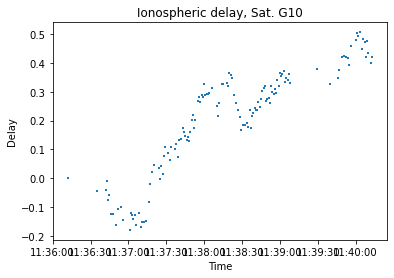
\includegraphics[width=1\textwidth]{./Figures/iono_G10.png}
			\caption {Délai (m) ionosphérique sur G10}
		\end{figure}
	\end{column}
	\end{columns}
\end{frame}

\section{Multipath}
\begin{frame}{Multipath}
	\begin{columns}
		\begin{column}{0.5\textwidth}
			\textbf{Multipath :} 
			%Le multipath est un phénomène de propagation d'onde radio qui se propage sur plusieurs trajets entre l'émetteur et le récepteur.
			Plusieurs trajets entre l'émetteur et le récepteur d'une même onde.
			\newline
			\newline
			Le multipath s'estime par : $MP = P - (\frac{2}{\alpha - 1} + 1) \cdot L_1 + \frac{2}{\alpha - 1} \cdot \L_2$
			\begin{flushright}
				\tiny{(Voir Démonstration Annexe 4)}
			\end{flushright}
			{\small \textbf{avec} $P$ la phase, $L_1$ la pseudorange, $L_2$ la pseudorange sur la deuxième fréquence et $\alpha$ le coefficient de réflexion.}
		\end{column}
		\begin{column}{0.5\textwidth}
			\begin{figure}
				\centering
				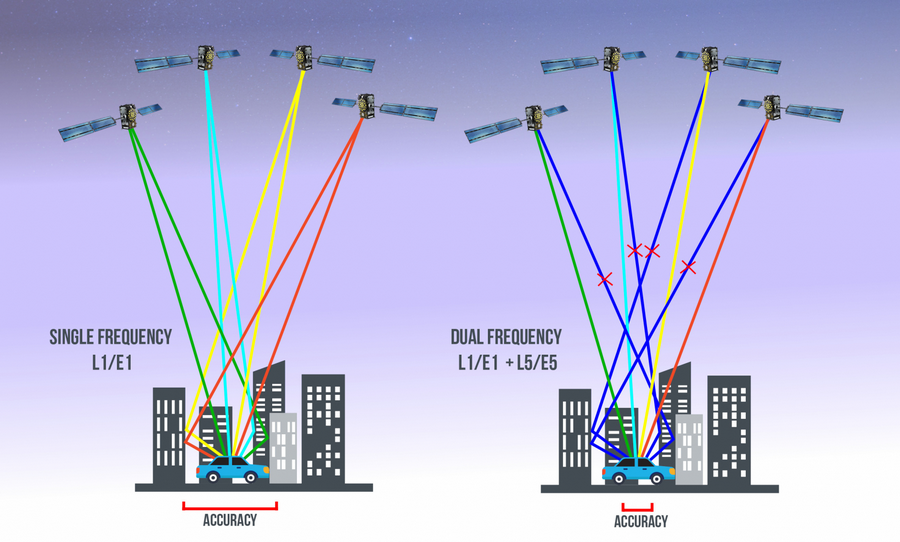
\includegraphics[width=0.9\textwidth]{./Figures/multipath2.png}
				\caption {Multipath \cite{esa}}	
			\end{figure}
			Besoin de la \textbf{phase} et de la \textbf{pseudorange} sur deux fréquences.
		\end{column}	
	\end{columns}
\end{frame}

\begin{frame}{Quelle erreur ?}
\begin{columns}
	\begin{column}{0.5\textwidth}
		\begin{figure}
			\centering
			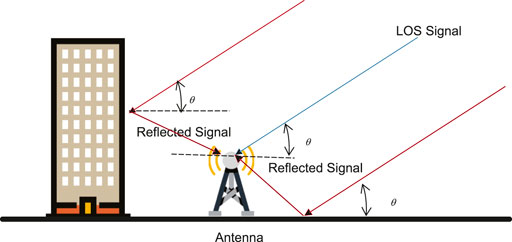
\includegraphics[width=0.8\textwidth]{./Figures/mp.jpg}
			\caption {Description du multipath \cite{10.3389/fphy.2022.1071539}}
		\end{figure}
		L'erreur est de \textbf{plusieurs mètres.} \cite{mperr}
	\end{column}
	\begin{column}{0.5\textwidth}
		\begin{figure}
			\centering
			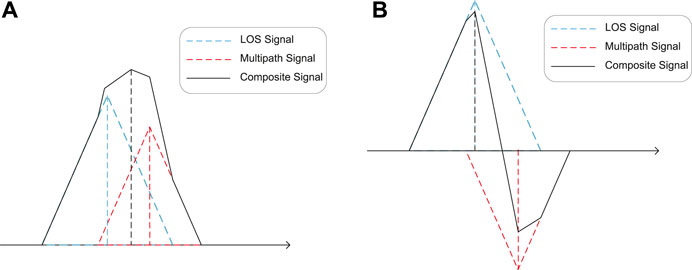
\includegraphics[width=0.7\textwidth]{./Figures/correl.jpg}
			\caption {Impact sur la fonction de corrélation {\tiny (\textit{Annexe 3})}}
		\end{figure}

		\begin{figure}
			\centering
			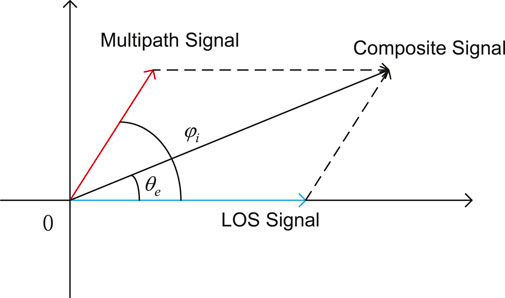
\includegraphics[width=0.7\textwidth]{./Figures/phase.jpg}
			\caption {Impact sur la phase}
		\end{figure}
	\end{column}
\end{columns}	
\end{frame}

\section{Exp. Multipath}
\begin{frame}
	\centering
	\begin{block}
		\scshape
		\begin{center}
			\Huge Expérimentations Multipath
		\end{center}
	\end{block}
\end{frame}

\begin{frame}{Protocole expérimental}
	\begin{itemize}
		\item Calcul du multipath à partir de la phase et de la pseudorange.
		\item Basé sur un article de Umberto et al. \cite{mi8}
		\begin{itemize}
			\item Utilisation d'un \textit{Xiaomi mi 8} et de \textit{Google GNSS Logger} pour récupérer les fichiers RINEX. {\tiny (voir Annexe 5)}
			\item Deux cas, peu de réflexion (campagne) et beaucoup de réflexion (ville).
			\item Traitement des données avec \textit{rtklib}. (Conversion de format)
			\item Traitement et calcul du multipath avec \textit{Tecq}.
			\item Analyse des résultats avec \textit{Python}. {\tiny (Voir Annexe 7)}
		\end{itemize}
	\end{itemize}
	\begin{columns}
		\begin{column}{0.3\textwidth}
			\begin{figure}
				\centering
				
\includegraphics[width=0.5\textwidth]{./Figures/rtklib.jpg}
				\caption {Outil de calcul de solution, \textit{rtklib}}
			\end{figure}		
		\end{column}

		\begin{column}{0.3\textwidth}
			\begin{figure}
				\centering
				
\includegraphics[width=0.7\textwidth]{./Figures/UNAVCO.png}
				\caption {Outil de calcul de multipath, \textit{Tecq}}
			\end{figure}
		\end{column}

		\begin{column}{0.3\textwidth}
			\begin{figure}
				\centering
				
\includegraphics[width=0.4\textwidth]{./Figures/gnss_logger.jpg}
				\caption {Outil de récupération de données, \textit{Google GNSS Logger}}
			\end{figure}
		\end{column}
	\end{columns}
\end{frame}

\begin{frame}{Résultats}
	Erreur multipath en ville et en campagne; statique.
	\newline
	\begin{columns}
		\begin{column}{0.5\textwidth}
			{\small En \textbf{ville}, on a une erreur de \textbf{2.5 mètres} en moyenne. \cite{mi8}}
			\begin{figure}
				\centering
				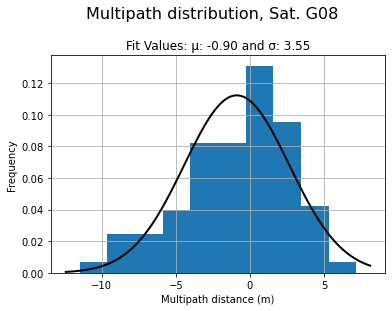
\includegraphics[width=0.8\textwidth]{./Figures/MP_G08_dis.png}
				\caption {Multipath de G08, erreur $(1 \pm 7)m$}
			\end{figure}
			% \begin{figure}
			% 	\centering
			% 	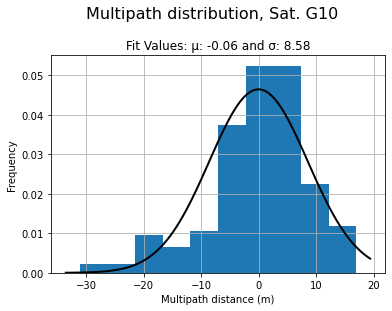
\includegraphics[width=0.4\textwidth]{./Figures/MP_G10_dis.png}
			% 	\caption {Multipath en extérieur}
			% \end{figure}
		\end{column}

		\begin{column}{0.5\textwidth}
			{\small En \textbf{campagne}, l'erreur est de \textbf{quelques dizaine de centimètres}. \cite{mi8}}
			\begin{figure}
				\centering
				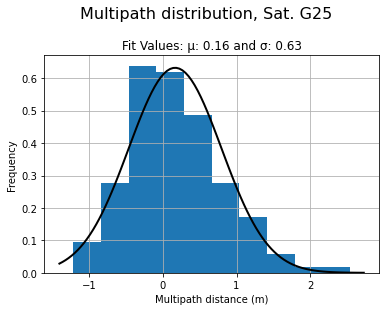
\includegraphics[width=0.8\textwidth]{./Figures/MP_G25_dis_camp.png}
				\caption {Multipath en extérieur, erreur $(0.2 \pm 1.2)m$}
			\end{figure}
			%\textit{J'ai pas encore les résultats, mais ça arrive.}
		\end{column}
	\end{columns}
\end{frame}

\section{Corrections}
\begin{frame}
	\frametitle{Corrections}
	Avec \textbf{RTKlib}:
	\newline
	\begin{columns}
		\begin{column}{0.5\textwidth}
			{\small \textbf{Sans} correction liée à la double fréquence (soit, \textit{ionosphère et multitrajets})\\
			Uniquement sur le \textbf{code} (pseudorange)}
			\begin{figure}
				\centering
				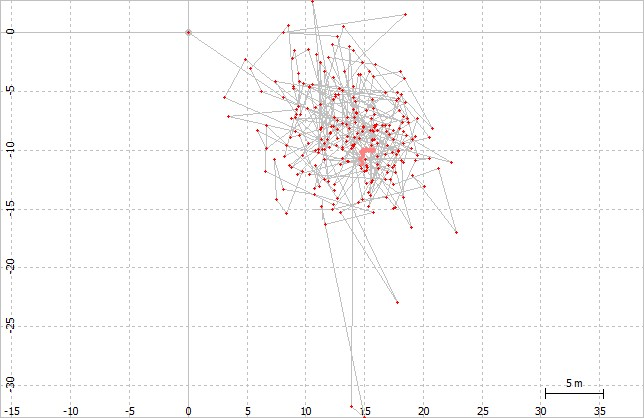
\includegraphics[width=0.8\textwidth]{./Figures/single_city.jpg}
				\caption {Calcul statique (Single), 5 m}
			\end{figure}
		\end{column}

		\begin{column}{0.5\textwidth}
			{\small \textbf{Avec} correction liée à la double fréquence. \cite{esa}\\
			Sur \textbf{pseudorange et phase}.}
			\begin{figure}
				\centering
				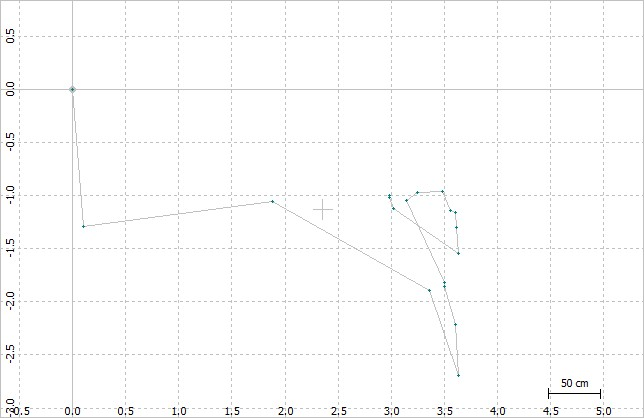
\includegraphics[width=0.8\textwidth]{./Figures/ppp_city.jpg}
				\caption {Calcul statique (PPP), 50 cm}
			\end{figure}
		\end{column}
	\end{columns}

\end{frame}

\section{Dilution géométrique}
\begin{frame}{Outils}
	\centering
	\textbf{Outils :} gnssplanning.com, calcul le GDOP.
	\newline
	\begin{columns}
		\begin{column}{0.5\textwidth}
			\begin{figure}
				\centering
				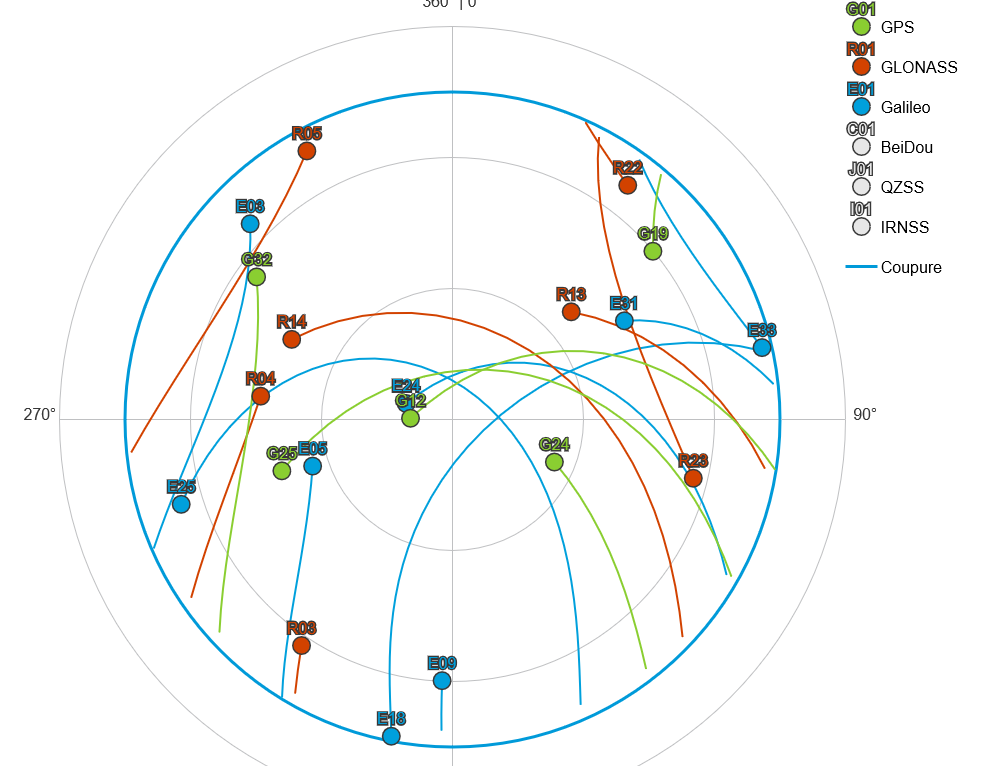
\includegraphics[width=0.7\textwidth]{./Figures/gdop15.png}
				\caption{Skyplot pour une limite de 15° (22/01/23 15h), GDOP: 2.35}	
			\end{figure}
		\end{column}

		\begin{column}{0.5\textwidth}
			\begin{figure}
				\centering
				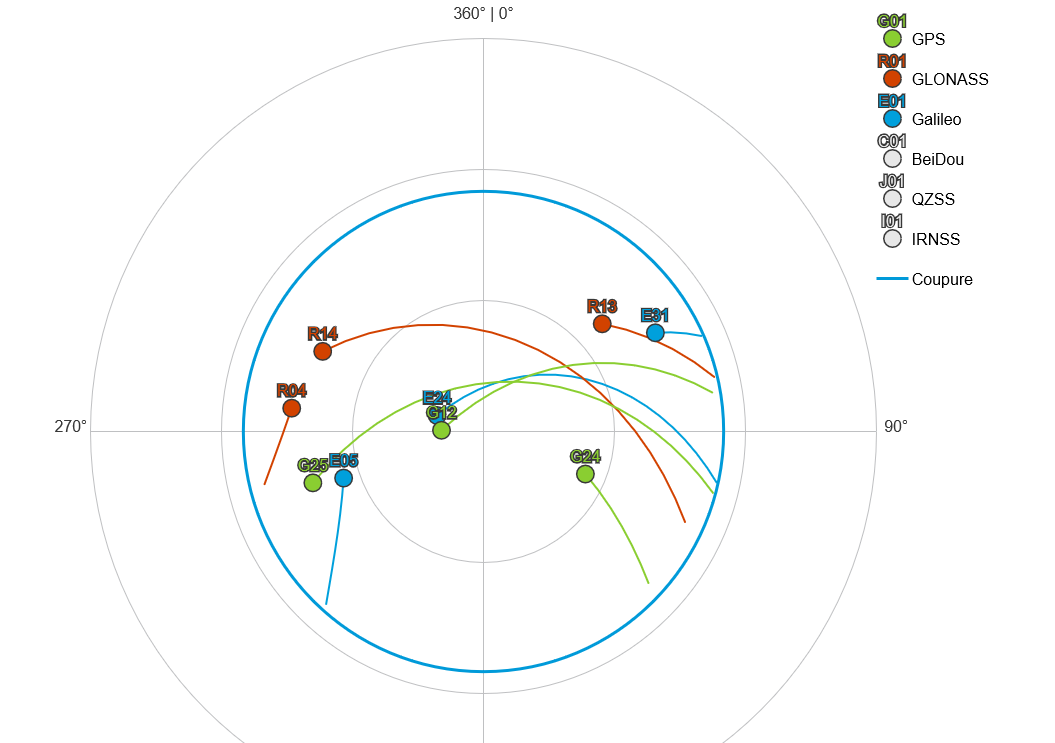
\includegraphics[width=0.8\textwidth]{./Figures/gdop35.png}
				\caption{Skyplot pour une limite de 35° (22/01/23 15h), GDOP: 4.56}	
			\end{figure}
		\end{column}
	\end{columns}
\end{frame}
\begin{frame}{Expérimentations}
	\textbf{Calcul de la position} à l'aide de \textit{RTKlib} avec un mask de 15° et 35°.
	\newline
	\begin{columns}
		\begin{column}{0.5\textwidth}
			\begin{figure}
				\centering
				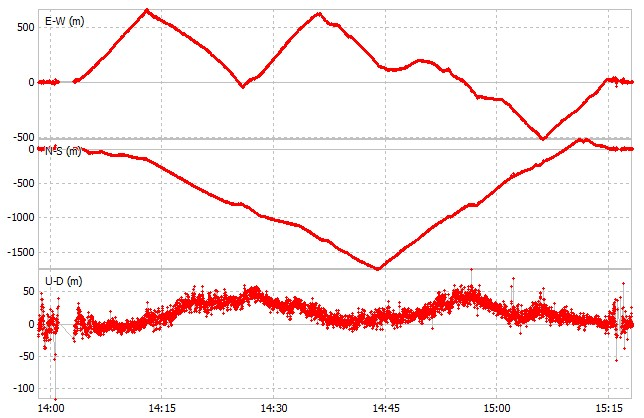
\includegraphics[width=0.8\textwidth]{./Figures/GDOP15.jpg}
				\caption{Position avec un mask de 15°}
			\end{figure}
		\end{column}

		\begin{column}{0.5\textwidth}
			\begin{figure}
				\centering
				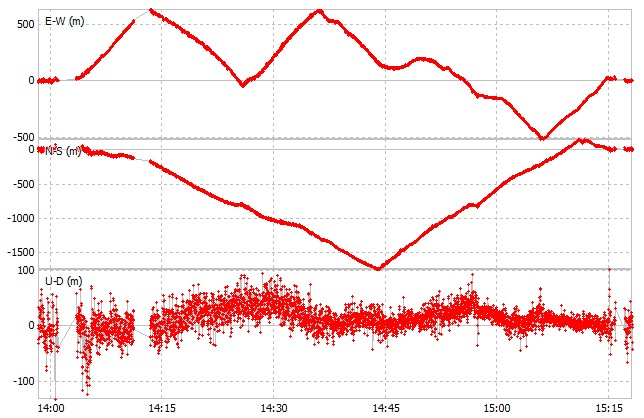
\includegraphics[width=0.8\textwidth]{./Figures/GDOP35.jpg}
				\caption{Position avec un mask de 35°}
			\end{figure}
		\end{column}
	\end{columns}
\end{frame}

\section{Conlusion}
\begin{frame}{Conclusion}
	Les smartphones multibandes, multi-constellation permettent d'améliorer la précision de la position:
	\begin{itemize}
		\item Une correction de l'erreur ionosphérique.
		\item En ville, grâce à la réduction du multipath.
		\item Le multi-constellation augmente le nombre de satellites utilisables, réduisant le GDOP.
	\end{itemize}
	Application commerciale possible : projet FLAMMINGO.
	\newline

	\textbf{Perspectives :} Solution RTK, PPP et augmenté par SBAS.\newline
	{\small (Voir début d'analyse dynamique en annexe)}
	\newline

	%Ainsi, les smartphones sont des outils de positionnement intéressants, mais peuvent devenir assez précis pour des applications de précision.
	%Ainsi diminuant le coût de l'infrastructure.
\end{frame}

\miniframesoff
\begin{frame}
	\centering
	\begin{block}
		\scshape
			\begin{center}
				{\Huge\emph{Merci de votre attention}} \newline
				\large Des Questions ?
			\end{center}
	\end{block}
\end{frame}

\miniframeson
\appendix
\begin{frame}[allowframebreaks]
	\frametitle{Bibliographie}
	\printbibliography
\end{frame}

\section{Annexe 1}
% \begin{frame}
% 	\label{appendix:1}
% 	\frametitle{Modélisation, perturbation gravitationnelle}
	
% \end{frame}

\begin{frame}{Élévation et SNR}
	\begin{figure}
		\centering
		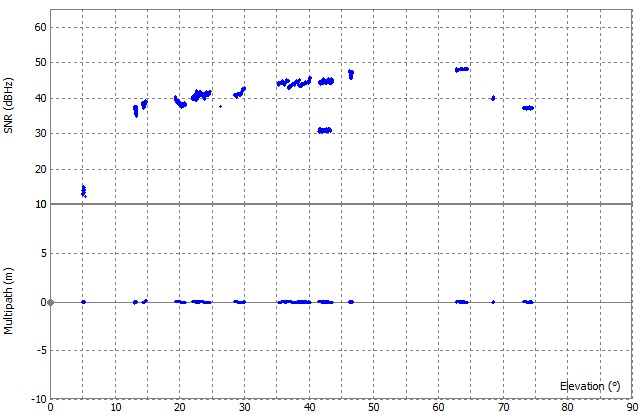
\includegraphics[width=0.8\textwidth]{./Figures/SNR_elev.jpg}
		\caption{Élévation et SNR}
	\end{figure}
\end{frame}

\section{Annexe 2}
\begin{frame}
	\label{appendix:2}
	\frametitle{Démonstration TEC}

	\begin{columns}
		\begin{column}{0.5\textwidth}
			{\small Modélisation de l'onde par: $\vec{\underline{E}} = \vec{\underline{E_0}} \cdot exp(i(\omega t - kx))$ \\
			\textbf{Hypothèses :} \\ Poids et champ magnétique négligeable devant le champ électrique.\\ 
			\textbf{PDF et passage en complexe :} $m_e \frac{d \vec{\underline{v_e}}}{dt} = -e \vec{\underline{E}} \leftrightarrow i m_e \omega \vec{\underline{v_e}} = -e \vec{\underline{E}}$
			\\ Par définition : $\vec{\underline{j_e}}= -e n_e \vec{\underline{v_e}}$, soit: $\vec{\underline{j_e}} = \frac{e^2 n_e}{i m_e \omega} \vec{\underline{E}}$ \\
			D'après l'équation de propagation : $\vec{\Delta} \vec E - \frac{1}{c^2} \frac{\partial^2 \vec E}{\partial t^2} = \mu_0 \frac{\partial \vec j}{\partial t}$ \\
			On en déduit le signal complexe : $k^2 = \frac{\omega^2}{c^2} - \frac{e^2 n_e}{c^2 \epsilon_0 m_e}$ \\
			\textbf{Vitesse de phase :} $v_{\phi} = \frac{\omega}{k} = \frac{c}{\sqrt{1 - \frac{{f_p}^2}{f^2}}}$ \\
			
			}
			\end{column}

		\begin{column}{0.5\textwidth}
				{\small \textbf{L'erreur de distance:} $L_1=c \tau_1$ \\
				Le retard: $\tau=\int_{0}^{H} \frac{dz}{v_g} - \int_{0}^{H} \frac{dz}{c} $ \\
				Ainsi le \textbf{retard} est : \boxed{\frac{1}{c} \int_{0}^{H} (\frac{c}{v_g} - 1)} \\
				On a que $v_g=v_{\phi} \cdot (1-\frac{f_p^2}{f_1^2})$ \\
				Soit: $L_1=\frac{a}{f_1^2} C_{ET}$ \newline

				\textbf{On a donc :} \newline}

				\boxed{C_{ET}=\int_{0}^{H}n_e dz = \frac{\tau}{a} \frac{f_1^2 f_5^2}{f_1^2 - f_5^2}}
			\begin{flushright}
				{\tiny \textit{D'après sujet E3A, \cite{e3a}}}
			\end{flushright}
		\end{column}
	\end{columns}
\end{frame}

\section{Annexe 3}
\begin{frame}
	\label{appendix:3}
	\frametitle{Le signal GPS}
	\begin{columns}
		\begin{column}{0.5\textwidth}
			Les récepteurs génèrent les fréquences porteuses L1 et L5 et compare avec celui reçu :
			\begin{figure}
				\centering
				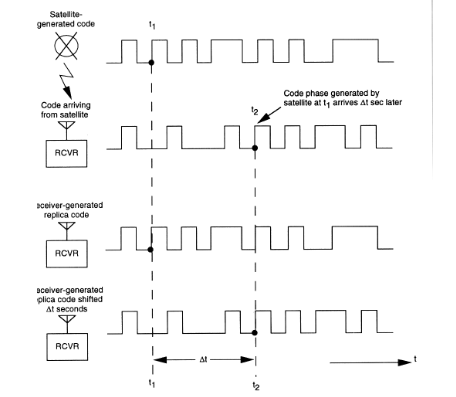
\includegraphics[width=0.8\textwidth]{./Figures/correl1.png}
				\caption {Décodage \cite{ens}}
			\end{figure}
		\end{column}
		\begin{column}{0.5\textwidth}
			{\tiny Détermine le pic de corrélation (code GOLD) et en déduit le décalage temporel.}
			\begin{figure}
				\centering
				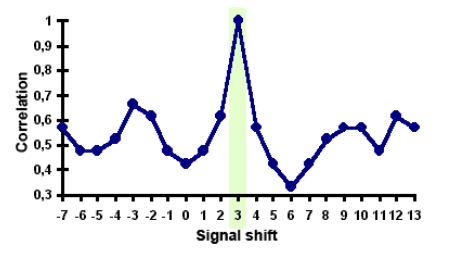
\includegraphics[width=0.5\textwidth]{./Figures/correl2.png}
				\caption {Fonction de corrélation \cite{ens}}
			\end{figure}

			\begin{figure}
				\centering
				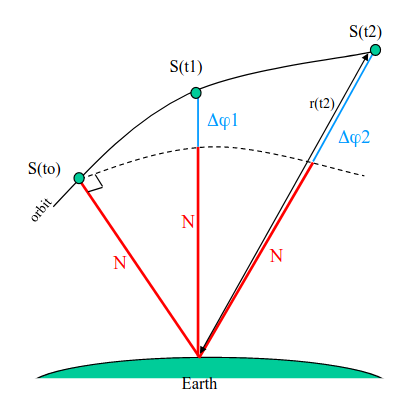
\includegraphics[width=0.4\textwidth]{./Figures/phase.png}
				\caption {Cycle de phase \cite{ens}}
			\end{figure}
		\end{column}
	\end{columns}
\end{frame}
\begin{frame}{Duty-Cycle}
	Ainsi comme le récepteur ne connait que le nombre de phases, il l'initialise à chaque fois.
	\newline
	Lorsque qu'il y a une interruption de signal, un nouveau cycle recommence.
	\begin{figure}
		\centering
		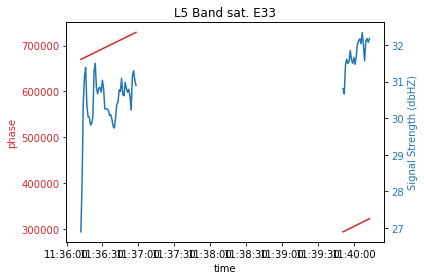
\includegraphics[width=0.6\textwidth]{./Figures/duty_cycle_eg.png}
		\caption{Exemple d'une interruption}
	\end{figure}
\end{frame}

\section{Annexe 4}
\begin{frame}
	\label{appendix:4}
	\frametitle{Démonstration Multipath}

	\begin{columns}
		\begin{column}{0.5\textwidth}
			{\small
			On \textbf{modélise les signaux} $L_1$ et $L_5$ par: \\
			$P_1 = R +I1 +MP1$ et $P_5 = R + I5 + MP5$ \\
			\textit{Avec : $R$ la distance réelle, $I1$ et $I5$ les erreurs ionosphériques, $MP1$ et $MP5$ les erreurs multipath.} \\
			Ainsi que leurs \textbf{phases respectives :} \\
			$L_1 = R - I1 + mp1 + B1$ et $L_5 = R - I5 + mp5 + B5$ \\
			\textit{Avec : $B1$ et $B5$ les ambiguïtés de phase. On néglige $mp << MP \leftrightarrow mp=0$} \\
			D'après \textit{Annexe 3} $I_i = \frac{A}{f_i^2}T_{EC}$ soit: 
			\begin{center}
				$\frac{I_5}{I_2} = \frac{f_1}{f_5}^2 = \alpha$
			\end{center}
			}
		\end{column}

		\begin{column}{0.5\textwidth}
			Après calcul des différentes combinaisons, \textbf{on obtient :} \\
			{\small $MP1 - P1 + (\frac{2}{\alpha - 1} + 1)L1 - (\frac{2}{\alpha - 1}) L5 = cte$} \\
			Comme le multipath est à valeur moyenne nulle, \textbf{on a :} \newline

			{\footnotesize \boxed{MP1 = P1 - (\frac{2}{\alpha - 1} + 1)L1 + (\frac{2}{\alpha - 1}) L5}} \newline

			\textbf{De même pour $MP5$ :} \newline
			
			{\footnotesize \boxed{MP5 = P5 - (\frac{2 \alpha}{\alpha - 1})L1 + (\frac{2 \alpha}{\alpha - 1} - 1)L5}} \\

			\begin{flushright}
				{\tiny \textit{D'après Eric Calais, \cite{ens}}}
			\end{flushright}
		\end{column}
	\end{columns}
\end{frame}
\begin{frame}
	\frametitle{Atténuation du multipath}

	\begin{columns}
		\begin{column}{0.5\textwidth}
			\begin{figure}
				\centering
				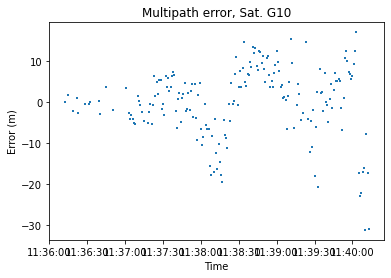
\includegraphics[width=1\textwidth]{./Figures/MP_G10.png}
				\caption{Multipath sur L1}
			\end{figure}
		\end{column}

		\begin{column}{0.5\textwidth}
			\begin{figure}
				\centering
				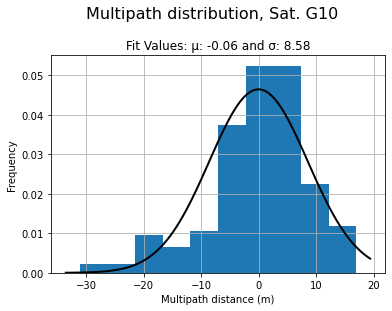
\includegraphics[width=1\textwidth]{./Figures/MP_G10_dis.png}
				\caption{Multipath sur L5}
			\end{figure}
		\end{column}
	\end{columns}

\end{frame}

\section{Annexe 5}
\begin{frame}
	\label{appendix:5}
	\frametitle{Fichiers RINEX}
	\textbf{RINEX} : Receiver Independent Exchange Format \\
	Fichier d'observation : \\
	\begin{itemize}
		\item Phase
		\item Code (Pseudorange)
		\item Doppler
		\item Rapport signal sur bruit (C/N0) 
	\end{itemize}
	Fichier de navigation : \\
	\begin{itemize}
		\item Ephémérides
		\item Heure
		\item Erreurs ionosphériques
		\item Erreurs de relativité restreinte
		\item ...
	\end{itemize}
\end{frame}

\begin{frame}[fragile, allowframebreaks]
	\frametitle{Exemple de fichier RINEX}

	Fichier de navigation :
	\begin{lstlisting}[basicstyle=\tiny]
2              NAVIGATION DATA                         RINEX VERSION / TYPE
CCRINEXN V1.6.0 UX  CDDIS               17-JAN-23 13:53     PGM / RUN BY / DATE 
IGS BROADCAST EPHEMERIS FILE                                COMMENT             
	0.2980D-07  0.2980D-07 -0.1192D-06  0.0000D+00          ION ALPHA           
	0.1516D+06 -0.1638D+06  0.0000D+00  0.6554D+05          ION BETA            
   -0.558793544769D-08-0.177635683940D-13   405504     2245 DELTA-UTC: A0,A1,T,W
	18                                                      LEAP SECONDS        
															END OF HEADER       
 1 23  1 17  0  0  0.0 0.223558396101D-03-0.466116034659D-11 0.000000000000D+00
	0.850000000000D+02-0.782812500000D+02 0.394659296287D-08 0.400711955078D+00
   -0.396929681301D-05 0.122224817751D-01 0.587478280067D-05 0.515365424919D+04
	0.172800000000D+06-0.124797224999D-06-0.163560063383D+01 0.128522515297D-06
	0.989089047026D+00 0.281125000000D+03 0.937393524649D+00-0.806640742682D-08
   -0.222509268404D-09 0.100000000000D+01 0.224500000000D+04 0.000000000000D+00
	0.200000000000D+01 0.000000000000D+00 0.465661287308D-08 0.850000000000D+02
	0.165673000000D+06 0.400000000000D+01 0.000000000000D+00 0.000000000000D+00
2 23  1 17  0  0  0.0-0.626868102699D-03 0.227373675443D-11 0.000000000000D+00
	0.780000000000D+02-0.814375000000D+02 0.447197198987D-08-0.574309133343D+00
   -0.426545739174D-05 0.200936053880D-01 0.661425292492D-05 0.515369303703D+04
	\end{lstlisting}
\end{frame}
\begin{frame}[fragile]
	Fichier d'observation :
	\begin{lstlisting}[basicstyle=\tiny]
3.03           OBSERVATION DATA    M                   RINEX VERSION / TYPE
GnssLogger          Xiaomi 10           20230117 132006 UTC PGM / RUN BY / DATE
Google GnssLogger                                           MARKER NAME
G    8 C1C L1C D1C S1C C5Q L5Q D5Q S5Q                      SYS / #### / OBS TYPES
E    8 C1C L1C D1C S1C C5Q L5Q D5Q S5Q                      SYS / #### / OBS TYPES
E L5Q  0.00000                                              SYS / PHASE SHIFT
 C1C    0.000 C1P    0.000 C2C    0.000 C2P    0.000        GLONASS COD/PHS/BIS
															END OF HEADER
> 2023 01 17 13 20 06.9995244  0 28                      
G06                     -9106.87612      2273.16912        13.59612                     -6784.17911      1726.83711        11.19011
G10                      8004.38113     -2010.76113        19.12713                      5935.91711     -1433.92611        10.63511
G11                    -12882.26412      3222.43712        17.30012                                                                
G12  20136967.66714     -2423.03914       846.72914        28.16814                                                                
G15                     14170.13812     -3560.32412        15.63512                                                                
G17                     11523.98012     -2880.99612        16.73612                                                                
	\end{lstlisting}
	\textbf{Note :} Les données ont été tronquées pour des raisons de lisibilité.
	\textbf{Dataset complet : } \url{https://mega.nz/folder/dlRWAb5K#JNMzol3-uhl9gx0fF0147w}
\end{frame}

\section{Annexe 6}
\begin{frame}
	\label{appendix:6}
	\frametitle{Biais d'horloge - Xiaomi Mi 8}
	Exemple de biais d'horloge et de fréquence pour un récepteur Xiaomi Mi 8, expérimental.
	\newline
	\begin{columns}
		\begin{column}{0.5\textwidth}
			\begin{figure}
				\centering
				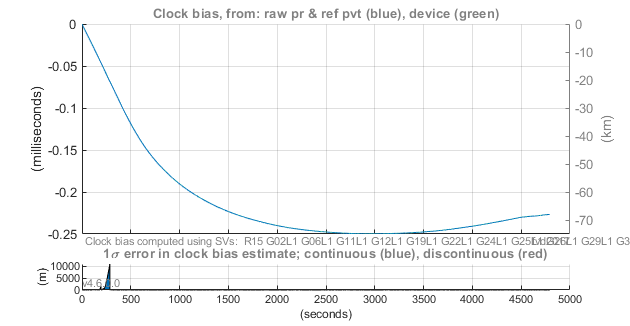
\includegraphics[width=1\textwidth]{./Figures/Clock bias.png}
				\caption {Biais d'horloge}
			\end{figure}
		\end{column}

		\begin{column}{0.5\textwidth}
			\begin{figure}
				\centering
				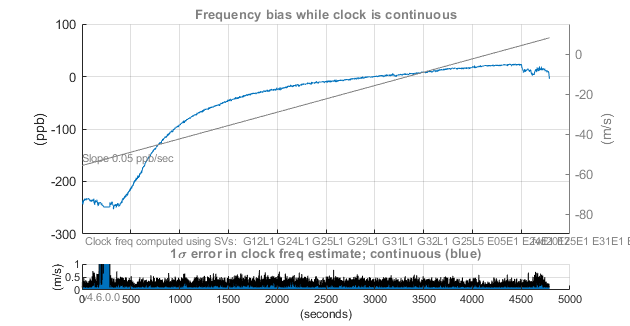
\includegraphics[width=1\textwidth]{./Figures/Clock bias_freq.png}
				\caption {Biais de fréquence}
			\end{figure}
		\end{column}
	\end{columns}
\end{frame}

\section{Annexe 7}
\begin{frame}[fragile, allowframebreaks]
	\frametitle{Code python - COMPACT3}
	\noindent
	\begin{lstlisting}[language=Python,basicstyle=\tiny]
import pandas as pd
from datetime import datetime, timedelta
nbval=0
sat=[]
def compread(filepath):
	file = open(filepath, "r")
	line = file.readline()
	i=1
	time=0
	cellsat=[]
	value=[]
	output=[['TIME', 'PRN', 'misure']]
	while line:
		if "GPS_START_TIME" in line:
			celldata=line.split()
			year=int(celldata[1])
			month=int(celldata[2])
			day=int(celldata[3])
			hour=int(celldata[4])
			minute=int(celldata[5])
			second=int(float(celldata[6]))
			dt=datetime(year, month, day, hour, minute, second)
		if (i % 2) != 0 and i>2:
			cellsat=line.split()
			time=int(float(cellsat[0]))
			if int(cellsat[1]) != -1:
				nbval=int(cellsat[1])
				sat=[cellsat[e] for e in range(2,nbval+2)]
		if (i % 2) == 0 and i>2:
			cellval=line.split()
			value=[]
			for f in range(nbval):
				if "S" in cellval[f]:
					value.append("NaN")
				else:
					value.append(float(cellval[f]))
				output.append([(dt+timedelta(seconds=time)),sat[f],value[f]])
		
		i=i+1
		line = file.readline()
	file.close()   
	return pd.DataFrame(output[1:], columns=output[0])
	\end{lstlisting}
	\textbf{Code complet :} \url{github.com/n005/tipe}
\end{frame}

\section{Annexe 8}
\begin{frame}
	\frametitle{Étude dynamique}
	\begin{columns}
		\begin{column}{0.5\textwidth}
			\begin{figure}
				\centering
				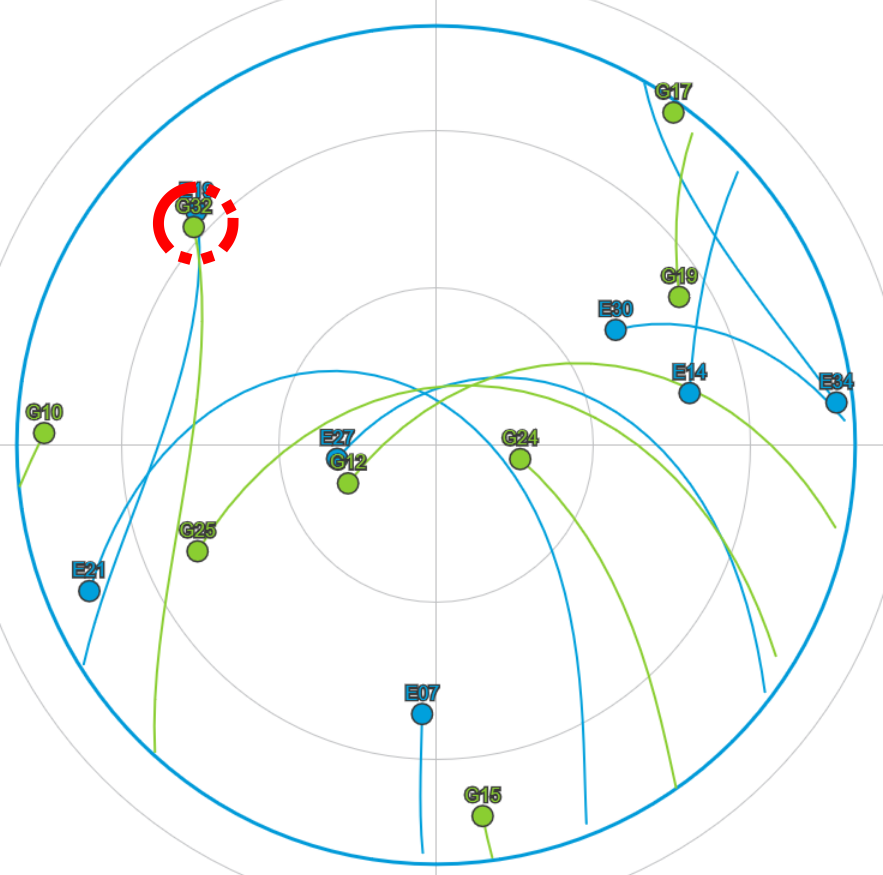
\includegraphics[width=0.7\textwidth]{./Figures/skyplot_dyn.png}
				\caption {Carte du ciel}
			\end{figure}
		\end{column}
		\begin{column}{0.5\textwidth}
			\begin{figure}
				\centering
				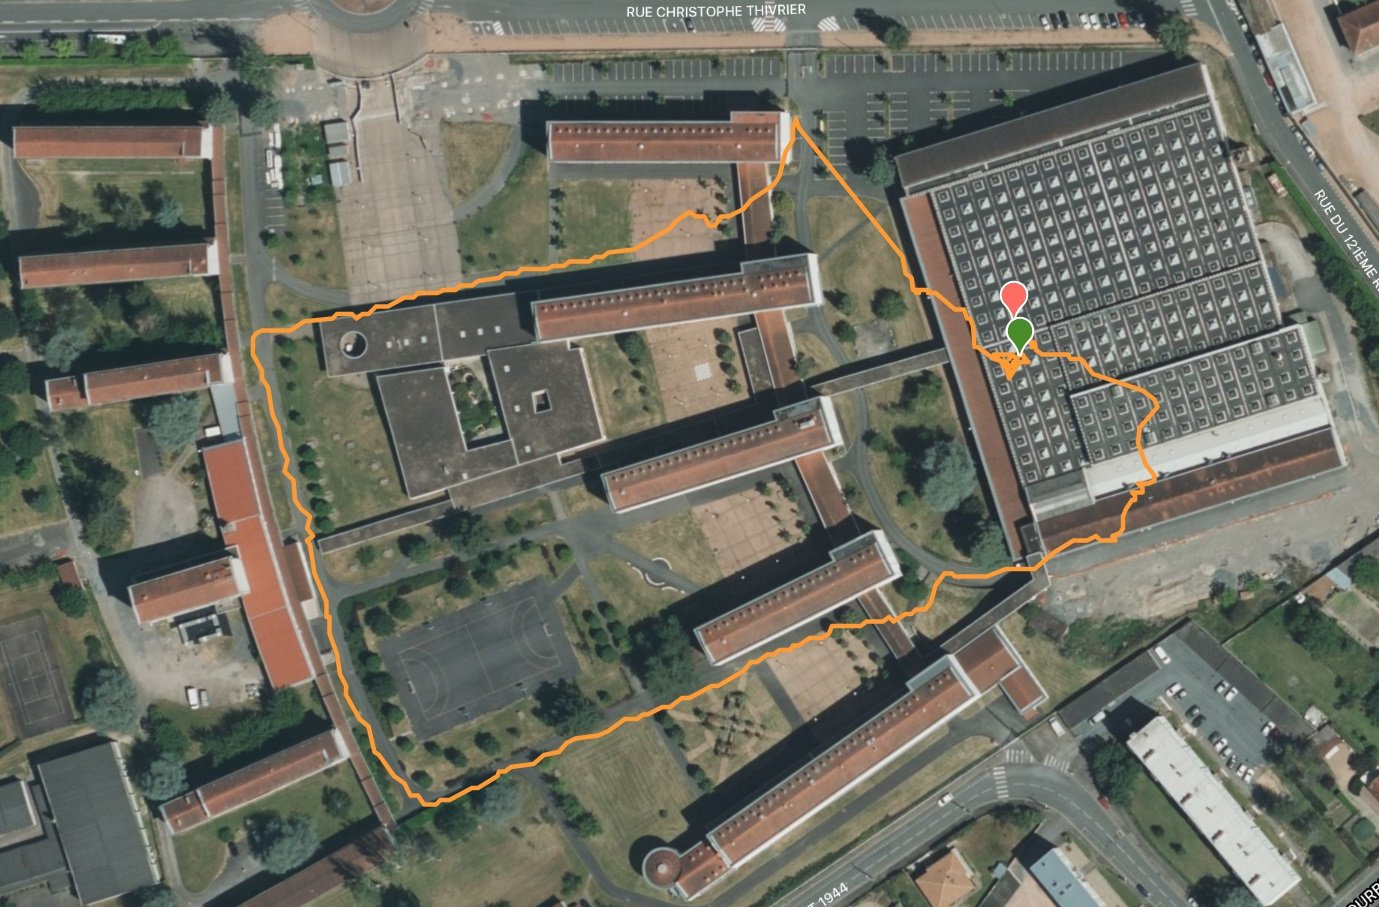
\includegraphics[width=0.5\textwidth]{./Figures/global_view.jpg}
				\caption {Vue Satellite}
			\end{figure}
			\begin{figure}
				\centering
				\includegraphics[width=0.7\textwidth]{./Figures/L1-G32.png}
				\caption {C/N0 L1 et phase G32}
			\end{figure}
		\end{column}
	\end{columns}
\end{frame}
\begin{frame}{Comparaison}
	\begin{figure}
		\centering
		\includegraphics[width=0.8\textwidth]{./Figures/ADR_vs_SpeudoR.jpg}
		\caption {Comparaison ADR(corrigé) et Pseudo-range}
	\end{figure}
\end{frame}
\begin{frame}{Réseau Centipede}
	Réseau RTK, permettant de faire du positionnement RTK (\textit{Real Time Kinematic}, Cinématique temps réel) et DGNSS(GNSS différentiel).
	\begin{columns}
		\begin{column}{0.5\textwidth}
			\begin{figure}
				\centering
				\includegraphics[width=0.3\textwidth]{./Figures/centipede.png}
				\caption {Logo - Centipede}
			\end{figure}
		\end{column}
		\begin{column}{0.5\textwidth}
			\begin{figure}
				\centering
				\includegraphics[width=0.8\textwidth]{./Figures/Centipede_map.png}
				\caption {Réseau Centipede}
			\end{figure}
			
		\end{column}
	\end{columns}
	Utilisation de RTKlib permettant de récupérer les données.
\end{frame}

\section{Annexe 9}
\begin{frame}{Outils - RTKlib}
	\begin{figure}
		\centering
		\includegraphics[width=0.9\textwidth]{./Figures/rtklib_over.jpg}
		\caption{RTKlib}
	\end{figure}
\end{frame}
\begin{frame}{Outils - GnssLogger}
	\begin{figure}
		\centering
		\includegraphics[width=0.25\textwidth]{./Figures/gnss_logger.png}
		\caption{GnssLogger}
	\end{figure}
\end{frame}

\section{Annexe 10}
\begin{frame}{Comparaison Ville-campagne}
	Résultats issue de l'étude de \cite{mi8}
	\begin{figure}
		\centering
		\includegraphics[width=0.8\textwidth]{./Figures/Umberto_results.png}
		\caption {Deux sites de mesures, a. campagne, b. ville}
	\end{figure}
\end{frame}
%--------- THANK YOU Text ------- texlive-most -------------------
%----------------------------------------------------
\end{document}
